%-------------------------------------------------------------------------------
\section{Computational Details}\label{Computational Details}
%-------------------------------------------------------------------------------
The \verb+respy+ package \citep{respy-1.0} provides the computational support for the project. Its online documentation is available at \url{http://respy.readthedocs.io} and thus I only outline the implementation details that are specific to this paper.

\paragraph{Optimization} I use the NEWUOA algorithm \citep{Powell.2006}. All tuning parameters are set to their default values. I use a diagonal scale-based preconditioner based on a gradient approximation. I set its minimum value to 0.00001.

\paragraph{Integration} The solution and estimation of the model produces two types of integrals. I need to determine $E\max$ during the solution step and simulate the choice probabilities to construct the sample log-likelihood. I evaluate both using Monte Carlo integration. I use 200 random draws for the choice probabilities.

\paragraph{Differentiation} The derivatives required for the preconditioning are approximated by forward finite differences with a step size of 0.0001.

\paragraph{Function Smoothing} I simulate the choice probabilities to evaluate the sample log-likelihood. With only a finite number of draws, there is always the risk of simulating zero probability for an agent's observed decision. So I use the logit-smoothed accept-reject simulator as suggested by \citet{McFadden.1989}. The scale parameter is set to 500.

\paragraph{Function Approximation} The details for the $E\max$ interpolation are already discussed in the text. However, there are some additional complications.
%
\begin{itemize}
\item Agents are only allowed to obtain 10 additional years of education. Thus, there exist a number of inadmissible states in late periods. However, $\bar{V}_3$ is still included in the interpolation regression and assigned an ad hoc penalty of -40,000. Results are not sensitive to the exact value as only about 5\% of the states in later periods are affected.
\item As noted in their correspondence with the editor, \citet{Keane.1994} drop the linear term of $V_3$ from the interpolation regression for the first parameterization due to reported collinearity problems. These are due to the small variation in the consumption value of schooling across states. I encounter the same problem and thus follow their lead.
\end{itemize}

I am indebted to several other open source tools among them \texttt{matplotlib} \citep{Matplotlib.2007} and \texttt{Vagrant} \citep{Hashimoto.2013}.
%-------------------------------------------------------------------------------
\subsection{Compute Machine}
%-------------------------------------------------------------------------------
\noindent This study utilized the high-performance computational capabilities of the Acropolis Linux cluster hosted by Social Sciences Computing Services at the University of Chicago. \path{Acropolis.uchicago.edu} is a clustered Linux system maintained by Social Science Computing Services at the University of Chicago. The head node contains 80 CPUs, 2 TB of memory and 110 TB of storage. The compute nodes provide and additional 1792 CPUs, 8 TB of memory, and 4 NVIDIA Tesla GPUs.
%-------------------------------------------------------------------------------
\subsection{Historical Perspective}\label{Appendix: Historical Perspective}
%-------------------------------------------------------------------------------
\citet{Keane.1994}'s work was particular valuable at the time because the computation power available was quite limited. For example, they report in a footnote that calculating the \textit{exact solution} for their prototypical model of occupational choice took roughly 50 minutes on a CRAY 2 supercomputer.
%
\begin{figure}[h!]
\caption{General Performance}\label{Appendix: General Performance}
\centering
\hspace{-1.5cm}\scalebox{0.30}{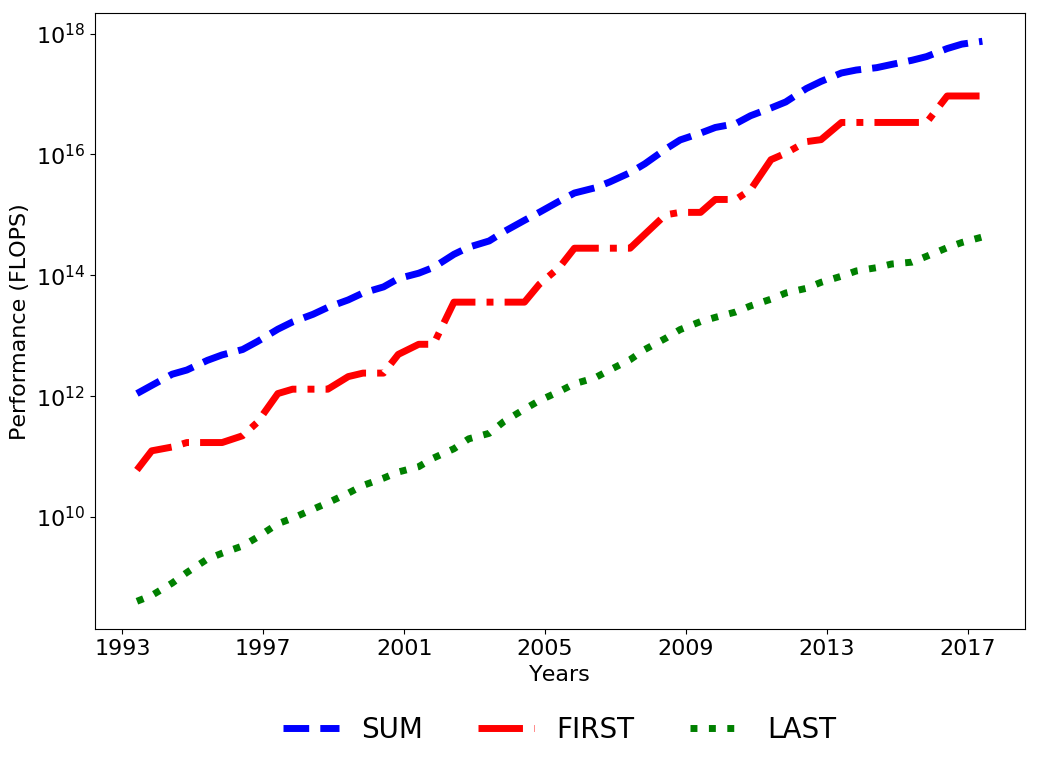
\includegraphics{../material/graph_performance_general.png}}\vspace{0.5cm}
\end{figure}

%
Since then the performance of supercomputers has grown exponentially. Figure \ref{Appendix: General Performance} illustrates the development of computing power over time for the world's fastest computer systems as measured by the TOP500 list \citep{TOP500.2017}. The number of floating point operations by the front runner has increased from 143 gigaflops in June 1994 to 93 petaflops 22 years later. Nowadays, the \textit{exact solution} to the model is calculated in about 8 minutes on the project's compute machine.
%
\begin{figure}[h!]
\caption{Performance for Model}\label{Appendix: Performance for Model}
\centering
\scalebox{0.30}{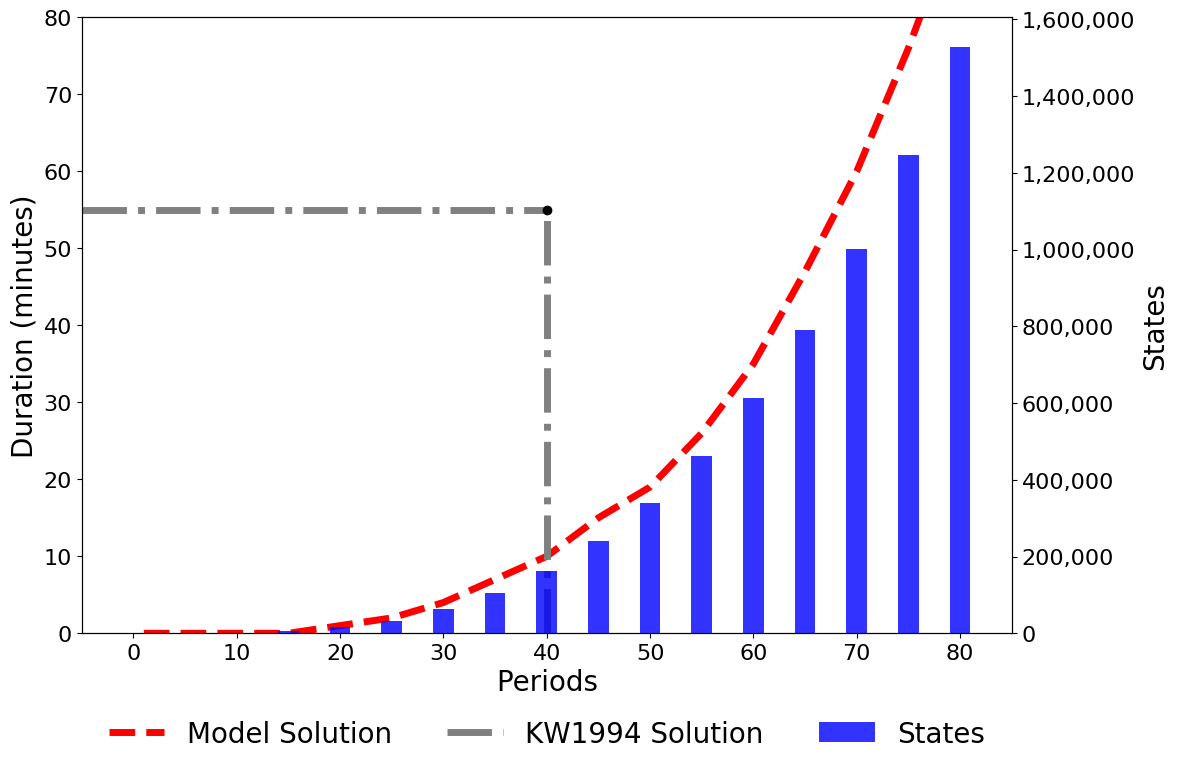
\includegraphics{../material/graph_performance_model.png}}\vspace{0.5cm}
\end{figure}

%
Figure \ref{Appendix: Performance for Model} shows the computation time for the \textit{exact solution} of the model for a varying number of time periods. Investing 50 minutes of CPU time now allows to solve the same model with 70 periods instead of 40. This entails are more than sixfold increase in the number of states from 163,410 to 1,001,520 states. This illustrates how structural econometricians will able to estimate and assess more and more realistic economic models as time goes by.
